\chapter{Evaluation}

\label{Chapter5}

\lhead{Chapter 5. \emph{Evaluation}}

In this chapter, the evaluation of the model is discussed with various techniques used to analyze how good the clustering has been done
and generation of the topics with other LLM models along with the human evalaution.

\section{Evaluation Design}
There are various techniques that can be used to evaluating the model performance and one of the most effective way is through human evaluation.
Along with this I have tried to evaluate the model performance by evaluating the clusters formed by the model amd comparing the topic generated
by the LLM model with other opensource LLM models. For the human evaluation following of the questions are asked to 

\begin{enumerate}
    \item\textbf{How well do you think notebooks effectively explain concepts or content to you?}
    
    This question was asked to check if the information provided to explain the Python codes for implemented models in the VS code Jupyter notebooks were easy to understand.

    \item\textbf{How would you rate the cluster formation of the model?}
    
    The purpose of this question is to determine whether the sentences inside the clusters that the model created were similar to one another or not.

    \item\textbf{How would you rate the topic generation of the model?}
    
    This question was asked in order to know if the topics generated by the model were good or not for the cluster sentences so that, the model was able to understand the content of the cluster
    and generate the proper topic name for the cluster.

    \item\textbf{How would you rate the LLM model approach when compared to the traditional approach?}
    
    This question will help us to understand if the LLM model approach is good or not compared to the traditional approach.
\end{enumerate}

\section{Cluster Evaluation}

Cluster evaluation is used to evaluate the quality of the clustering done by the model. There are various techniques that can be used to evaluate and
I have considered the below technique. This cluster evaluation is done using the Silhouette Score, Davies-Bouldin Index and Calinski-Harabasz Index which will
suitable for evaluating the clusters formed by the clustering algorithm. This will help to understand the quality of the clusters and embedding models.
As the data is in the German language, finding the embedding model is very important and the selected embedding model need to cover the entire data so that,
the clustering can be done properly. As if chosing a inefficient embedding model, will result in inproper cluster formation and which leds to the poor results.
So, by conducting theis evaluation, we can understand the quality of the embedding model along with the cluster formation. The below metrics will give an idea 
how the evalaution score is calculated is explained below,

\begin{enumerate}
    \item{\textbf{Silhouette Score:}} Measure of how closely an object is to one's cluster relative to other clusters. The score has a range from -1 to 1, with
    higher score indicating better clusters. These also give insights into the cluster cohesion and separation.
    
    \item{\textbf{Davies-Bouldin Index:}} ThThis indexes the average similarity between each cluster and its most similar one. Lower Davies-Bouldin values determine a better partition.
    The compactness of the separation of the clusters will be measured.
    
    \item{\textbf{Calinski-Harabasz Index:}}  It measures the ratio of between-cluster scatter to within-cluster scatter. Bigger values are indicative of a better-defined cluster.
    Index works best with clusters that are convex in shape \cite{geeksforgeeks_clustering_metrics}.
\end{enumerate}


\noindent The metrics for each embedding model are shown below,

\begin{table}[htbp]
    \centering

    \label{tab:cluster_metrics}
    \begin{tabular}{|l|c|c|c|}
    \hline
    \textbf{Embedding Model} & \textbf{Silhouette Score} & \textbf{Davies-Bouldin Index} & \textbf{Calinski-Harabasz Index} \\
    \hline
    Jina AI  de & ~(0.3 - 0.6) & ~0.95& ~3459 \\
    \hline
    Cross RoBERTa en-de & ~(0.1 - 0.4) & ~1.1 & ~456 \\
    \hline
    BERTopic & ~(-0.3 - 0.1) & ~1.5 & ~236 \\
    \hline

    \end{tabular}
    \caption{Cluster Evaluation Metrics for HDBSCAN}
\end{table}
\vspace{1cm}
Based on the above metrics, the Jina AI de model performed well with the hdbscan clustering for the german interview transcript dataset. 
This metric made me to choose the Jina AI de model for embedding of the interview transcripts.


\section{Topic Generation with other LLMs}

Evaluation includes my using the same LLM model for topic generation by feeding the clusters to the LLM model and prompting the model for
generating topics based on the cluster. Since I am using the Llama 3 - 8B model for topic generation, I want to check with other LLM models.
The topics generated for each cluster were manually evaluated for whether they are similar or not. Random proverb clusters chosen to prompt 
models like the GPT 3.5 model by Open AI ChatGPT, Google Gemini model, and a few other LLM models, have been presented here.

The evaluation was performed manually on the generated topics of each cluster to verify if it is similarly trained as the state-of-the-art models.
which will give an overview of how good the clustering has been done and what topics are generated.

The output of the complete text based on the sentences belong to the particular cluster will looks as shown in the below attached imaged,

\begin{figure}[htbp]
    \begin{center}
      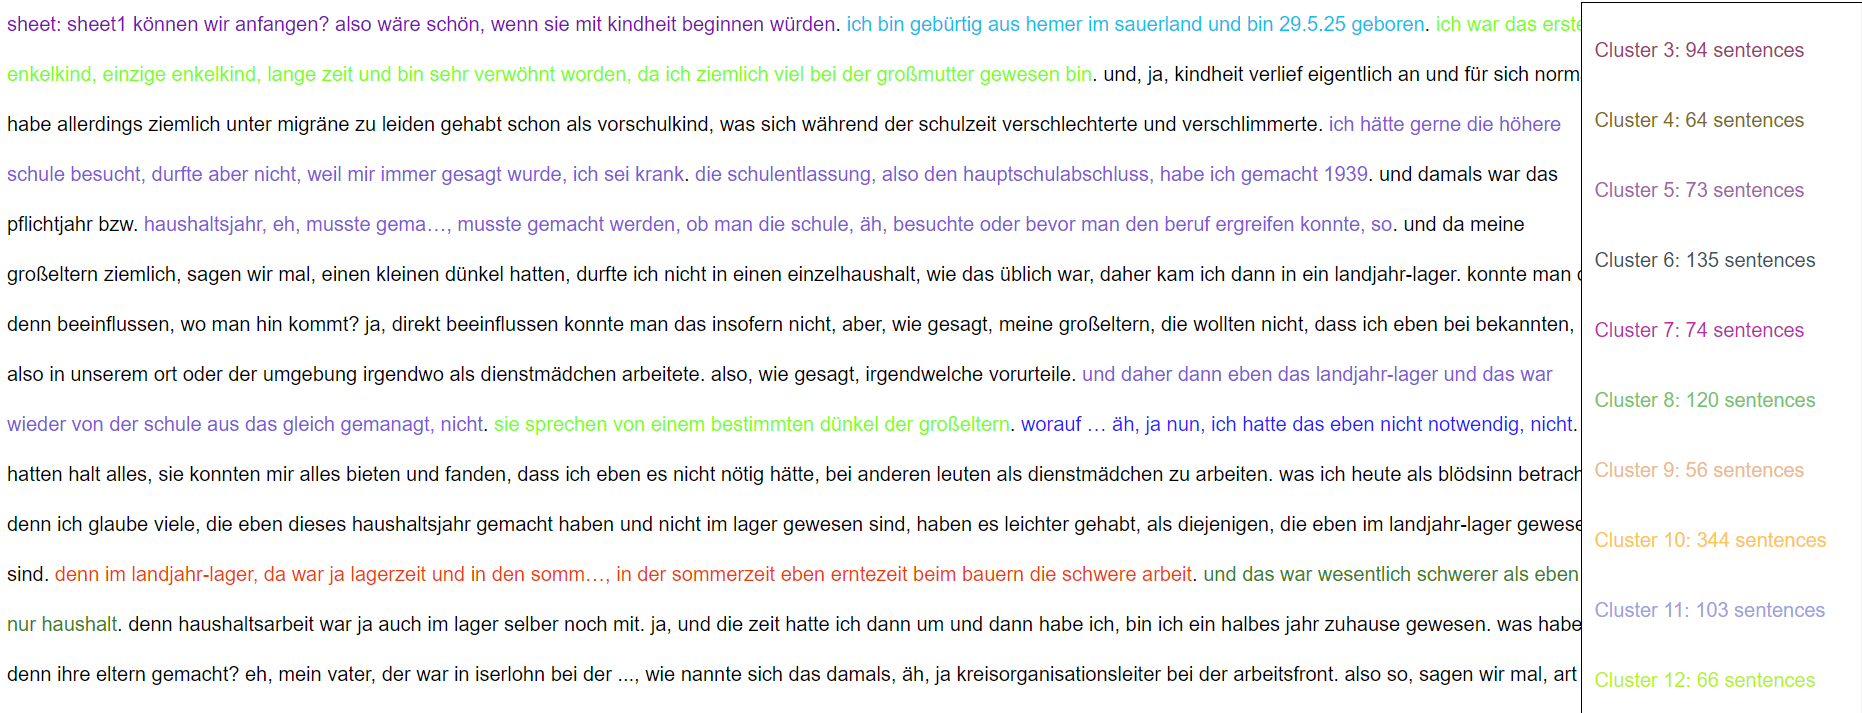
\includegraphics[width=12cm]{./Images/cluster_legends.png}
       \caption{Clusters sentence distribution w.r.t Original text corpus}
       \label{fig: Clusters sentence distribution w.r.t Original text corpus}
    \end{center}
\end{figure}

This will helps us to get to know how the sentences for each cluster are present and how the topics are distributed accross the documents.

\noindent Along with these metrics, I have also compared the clusters formed and the generated topics of the model with human estimation.
By taking feedback from humans, on the questions framed in the evalaution design section to understand the model performance.
\vspace{3cm}

\noindent\textbf{Human Feedback}

\noindent\textbf{On Q1:} As jupyter notebooks consist of python code with comment the people with the technical knowledge were able to understand the code without much explanation but, the people with 
non-technical knowledge were understanding the notebook code based on the comments added. So, the people with non-technical knowledge suggested to having a user interface would be better 
so that everyone can understand.

\noindent\textbf{On Q2:} As the data is huge and there are lot of sentences under each cluster, a random cluster was selected to people to get to know the whether the sentences in the cluster is similar or not 
and got positive feedback that, the sentence in the cluster is similar to each other and there are lot of sentences in the cluster which has same meaning but expressed in different ways.

\noindent\textbf{On Q3:} As a this question is a follow up of Q2, the topic generated by the model for the specific cluster is almost matching and the topic name generated is representing as the title of the cluster 
which will help to understand related to what domain the cluster belongs to.

\noindent\textbf{On Q4:} This question was asked to know if the LLM approach is good or not compared to the traditional approach where I tried to show output of the conventional approach like LDA, NMF etc.., and 
ask to compare with this thesis approach based on this there was some feedback like the traditional approach has the word representation and this model has a sentence representation. The traditional approach is 
has grouped the words which are like each other together and the LLM approach has a sentence representation. There was mixed feedback on this question as few people felt traditional approach is better and few people
felt the LLM approach is better.


Based on the above feedback, for Question 1, 2 \& 3, decide to build a web application which can handle the same text data. 


% \\\\\\\\\\\\\\\\\\\\\\\\\\\\\\\\\\
% section: discussion
%////////////////////////////////////
\section{Discussion}

After reciving the feedback from the humans on the evalaution of the models, it was clear that the Jina AI de model was performing well
with the HDBSCAN clustering algorithm for the interview transcripts dataset. As the feedback was positive, when it comes to the clustering of the sentences
and generation topic name of the cluster made it clear that the technique of achieving the topic modelling using embedding, cluster and LLM models was good.
Eventhrough, the feedback on the comparsiom of the traditional approach and LLM approach was mixed. Based on these feedbacks the idea of building an web application
came up and the web aplication was created which can handle the same text data (mentioned in the previous section).

The cluster evaluation plays an important role as it help to understand the quality of the clusters and embedding models.
The meteric scores of silhouette score, davies-bouldin score and calinski-harabasz score gave an idea of how good the clustering is done.
 The evaluation of the topic generation with other LLMs is a manual evaluation which also helped in understanding how good the Llama model 
 has generated the topics and along with the human feedback on the cluster formation and the topic generation help to understand the performance
 of the model. With the completion of this chapter, the evaluation of the models has been completed.The next chapter will provide a summary of the 
thesis and also explain the challenges encountered during the research.
